\begin{frame}{Example with Dependent Inputs} % How does it look?
    \begin{align*}
    y(x_1, x_2) = 2x_1 + x_2^{2} + x_1 x_2, \qquad \rho = 0.8
  \end{align*}
  \begin{columns}
    \column{0.5\textwidth}
      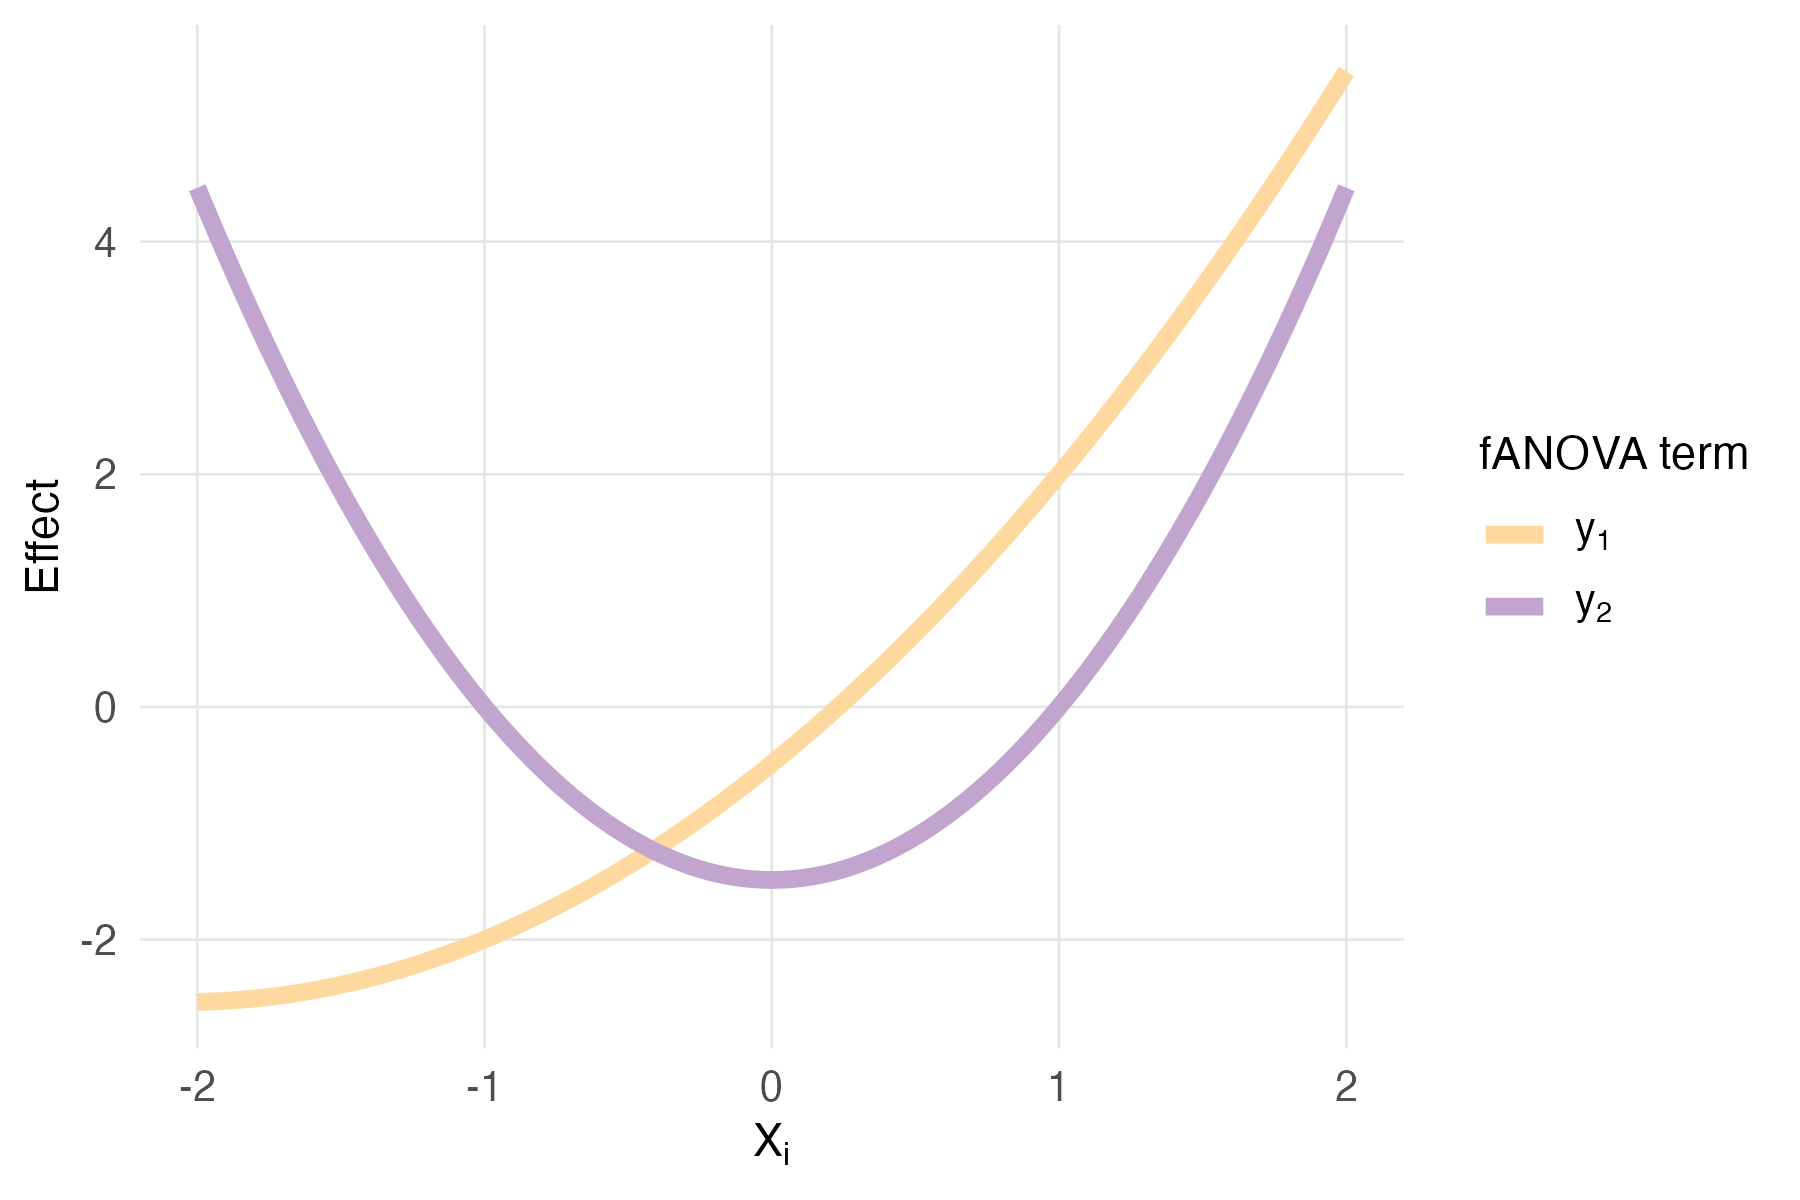
\includegraphics[width=\linewidth]{../images/experiment_section/gen_ex_1_a1p20_a2p00_a11p00_a22p10_a12p10_rhop08_main.png}
    \column{0.5\textwidth}
      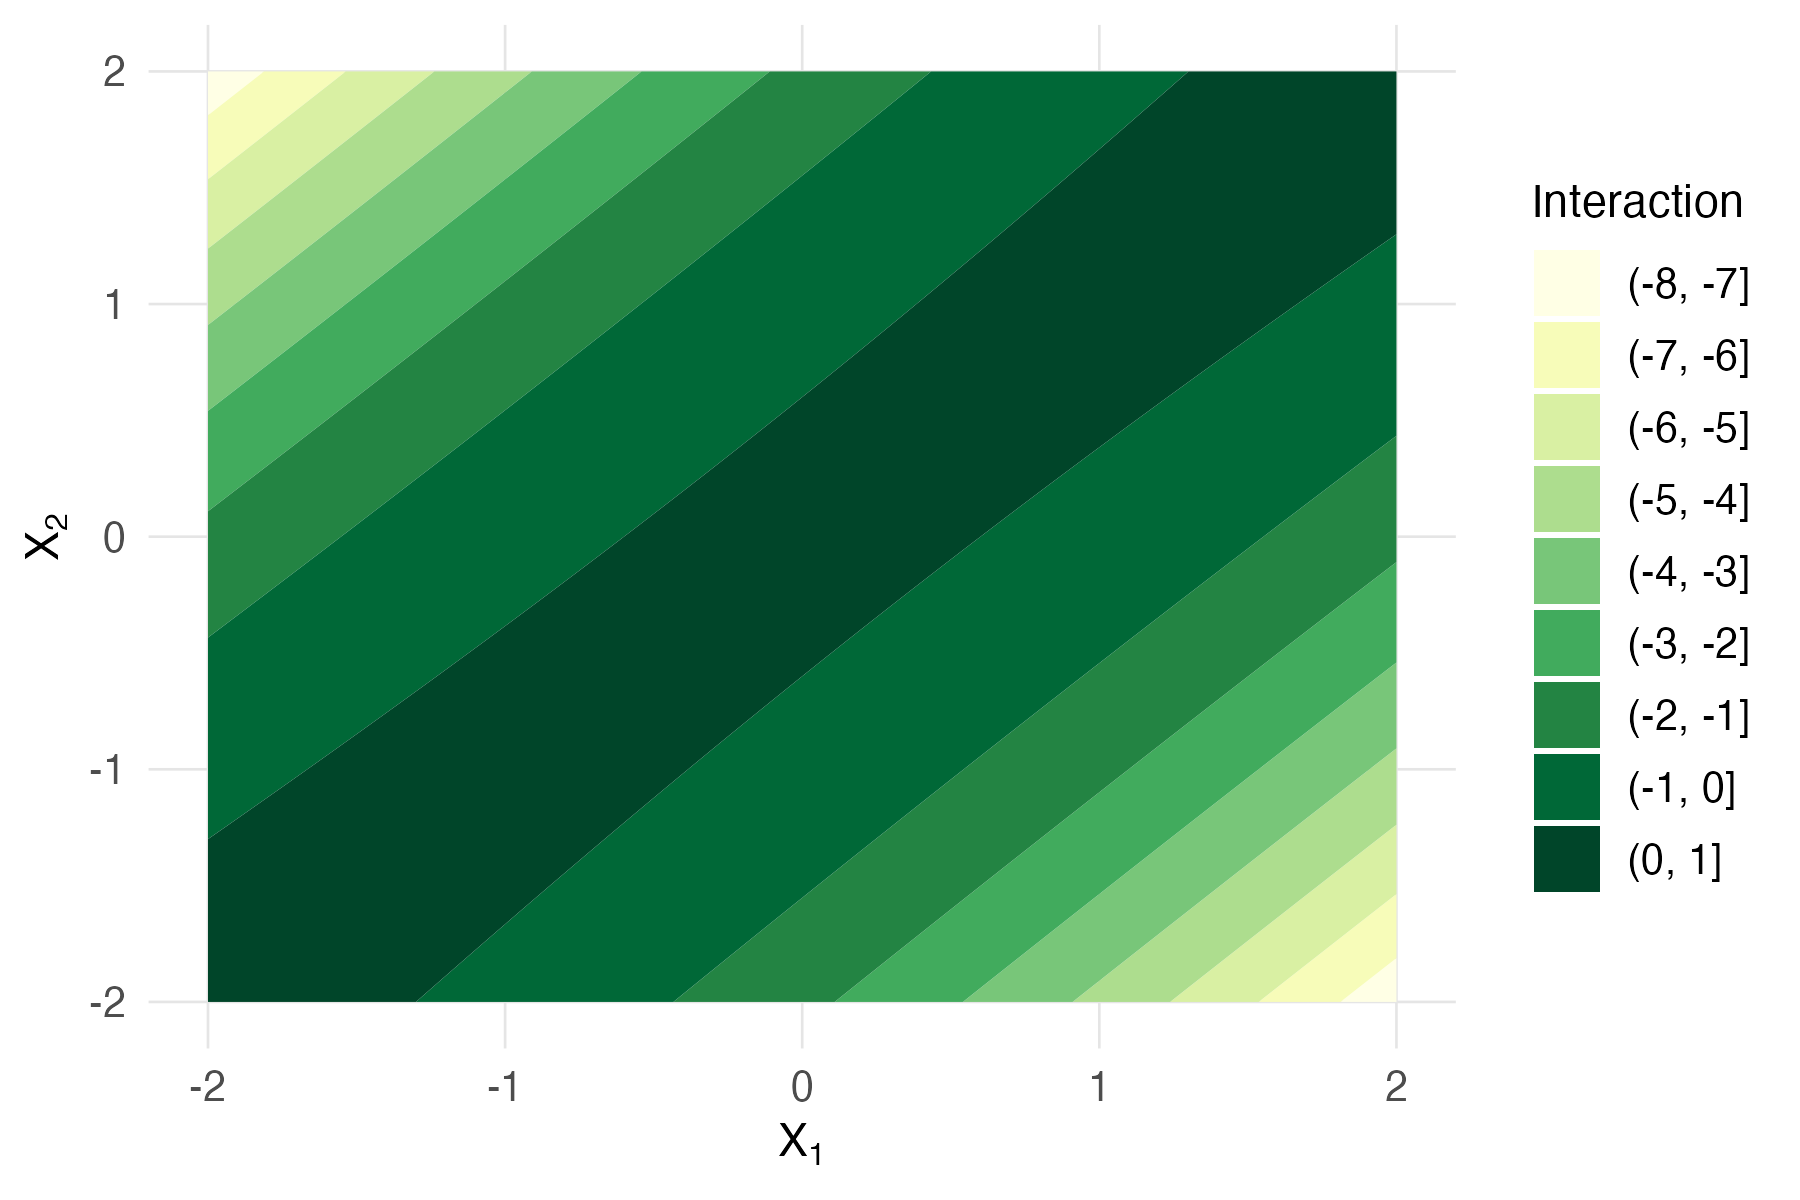
\includegraphics[width=\linewidth]{../images/experiment_section/gen_ex_1_a1p20_a2p00_a11p00_a22p10_a12p10_rhop08_interaction.png}
  \end{columns}
\end{frame}

%==================================================
% Slide 2 – Conditions (Weaker Annihilating Conditions)
%==================================================
\begin{frame}{Weaker Annihilating Conditions}
  \begin{block}{Weak Annihilating Conditions}
    \[
      \int_{\mathbb{R}} y_{u, G}(\boldsymbol{x}_u) f_{\boldsymbol{X}_u}(\boldsymbol{x}_u) d\nu (x_i) = 0 \quad \text{for} \quad i \in u \neq \emptyset.
    \]
  \end{block}
  \begin{itemize}
    \item Allows dependent input distributions
    \item Leads to hierarchical orthogonality
  \end{itemize}
    \[
  \mathbb{E}[y_{u, G}(\boldsymbol{X}_u)] := \int_{\mathbb{R}^N} y_{u, G}(\boldsymbol{x}_u) f_{\boldsymbol{X}}(\boldsymbol{x}) \, d\nu (\boldsymbol{x}) = 0.
  \]
  \[
  \mathbb{E}[y_{u, G}(\boldsymbol{X}_u)y_{v, G}(\boldsymbol{X}_v)] := \int_{\mathbb{R}^N} y_{u, G}(\boldsymbol{x}_u) y_{v, G}(\boldsymbol{x}_v) f_{\boldsymbol{X}}(\boldsymbol{x}) \, d\nu (\boldsymbol{x}) = 0.
  \]
\end{frame}


%==================================================
% Slide 4 – Construction
%==================================================
\begin{frame}{Component Definition (Coupled System)}
  \begin{align*}
    y_{\emptyset,G} 
      &= \int_{\mathbb{R}^N} y(\boldsymbol{x}) f_{\boldsymbol{X}}(\boldsymbol{x}) \, d \nu(\boldsymbol{x}) \\[3ex]
    y_{u,G}(\boldsymbol{X}_u) 
      &= \int_{\mathbb{R}^{N - |u|}} y(\boldsymbol{X}_u, \boldsymbol{x}_{-u}) 
         f_{-u}(\boldsymbol{x}_{-u}) \, d \nu(\boldsymbol{x}_{-u})
         - \sum_{v \subsetneq u} y_{v,G}(\boldsymbol{X}_v) \\ 
      &\quad - \!\!\!\!\!\!\sum_{\substack{\emptyset \ne v \subseteq \{1,\dots,N\} \\ 
         v \cap u \ne \emptyset,\ v \not\subset u}} 
         \int_{\mathbb{R}^{|v \cap -u|}} 
         y_{v,G}(\boldsymbol{X}_{v \cap u}, \boldsymbol{x}_{v \cap -u}) 
         f_{v \cap -u}(\boldsymbol{x}_{v \cap -u}) \, 
         d \nu(\boldsymbol{x}_{v \cap -u})
  \end{align*}
\end{frame}

\begin{frame}{Component Definition (Coupled System)}
\begin{align*}
    % --- constant term (always visible)
    y_{\emptyset,G} 
      &= \int_{\mathbb{R}^N} y(\boldsymbol{x}) 
         f_{\boldsymbol{X}}(\boldsymbol{x}) \, d \nu(\boldsymbol{x}) \\[3ex]
    % --- nonconstant formula (appears from slide 2 onward)
    \onslide<2->{%
    y_{u,G}(\boldsymbol{X}_u) 
      &= \int_{\mathbb{R}^{N - |u|}} 
         y(\boldsymbol{X}_u, \boldsymbol{x}_{-u})
         f_{-u}(\boldsymbol{x}_{-u})\, d \nu(\boldsymbol{x}_{-u}) 
         \textcolor<3->{pastelBlue}{-\sum_{v \subsetneq u} y_{v,G}(\boldsymbol{X}_v)} \\ 
      &\quad 
        \textcolor<4->{pastelRed}{
        -\!\!\!\!\!\!\sum_{\substack{\emptyset \ne v \subseteq \{1,\dots,N\} \\ 
        v \cap u \ne \emptyset,\ v \not\subset u}} 
        \int_{\mathbb{R}^{|v \cap -u|}} 
        y_{v,G}(\boldsymbol{X}_{v \cap u}, \boldsymbol{x}_{v \cap -u}) 
        f_{v \cap -u}(\boldsymbol{x}_{v \cap -u}) 
        \, d \nu(\boldsymbol{x}_{v \cap -u})}
    }% end onslide<2->
  \end{align*}

  \begin{columns}[t]
    % --- Left Venn diagram (appears at overlay 2)
    \begin{column}{0.48\textwidth}
      \centering
      \only<3->{
        \begin{tikzpicture}[scale=0.6]
          \draw[black, thin] (-1.5,-1.5) rectangle (4,2) 
                node[anchor=north east] {$\mathbb{N}$};
          \draw[thick,pastelBlue] (1.2,0.2) ellipse (2.0cm and 1.2cm);
          \node[pastelBlue] at (-0.1,0.8) {$u$};
          \draw[thick,pastelBlue] (1.2,0.2) ellipse (1.0cm and 0.6cm);
          \node[pastelBlue] at (0.8,0.2) {$v$};
        \end{tikzpicture}
      }
    \end{column}
    % --- Right Venn diagram (appears at overlay 3)
    \begin{column}{0.48\textwidth}
      \centering
      \only<4->{
        \begin{tikzpicture}[scale=0.6]
          \draw[black, thin] (-1.5,-1.5) rectangle (4,2) 
                node[anchor=north east] {$\mathbb{N}$};
          \draw[thick,pastelRed] (0.5,0.2) ellipse (1.7cm and 1.2cm);
          \node[pastelRed] at (-0.2,0.2) {$u$};
          \draw[thick,pastelRed] (2.0,0.2) ellipse (1.7cm and 1.2cm);
          \node[pastelRed] at (2.7,0.2) {$v$};
          \node[pastelRed] at (1.2,0.2) {$u \cap v$};
        \end{tikzpicture}
      }
    \end{column}
  \end{columns}
\end{frame}


\begin{frame}
    \begin{itemize}
    \item $N = 3$, $u = \emptyset$
  \end{itemize}
    \begin{equation*}
    y_{\emptyset,G} = \mathbb{E}[y(\boldsymbol{X})]
    \end{equation*}
    \begin{itemize}
      \item $u = \{1\}$ $\rightarrow$ $v \subsetneq u = \emptyset$ and $(\emptyset \ne v \subseteq \{1,\dots,N\},\ v \cap u \ne \emptyset,\ v \not\subset u) = \{1,2\}, \{1,2,3\}$
    \end{itemize}
    \begin{align*}
       y_{{\{1\}},G}(\boldsymbol{X}_u) &= \int_{\mathbb{R}^{2}} y(x_1, x_2, x_3) f_{{\{2, 3\}}}(x_2, x_3) \, d \nu(x_2, x_3) - y_{\emptyset,G} \\[1em]
    &\quad - \int_{\mathbb{R}}y_{{\{1, 2\}}, G}(x_1, x_2)f_{{\{2\}}}(x_2) \, d \nu(x_2) - \int_{\mathbb{R}}y_{{\{1, 3\}}, G}(x_1, x_3)f_{{\{3\}}}(x_3) \, d \nu(x_3) \\[1em]
    &\quad - \int_{\mathbb{R}^2}y_{{\{1, 2, 3\}}, G}(x_1, x_2, x_3)f_{{\{2, 3\}}}(x_2, x_3) \, d \nu(x_2, x_3)
    \end{align*}
  \end{frame}

\begin{frame}{Construct components via Fourier-polynomial expansion}
    \begin{align*}
y(x_1,x_2) 
&= a_0 + a_1 x_1 + a_2 x_2 
   + a_{11} x_1^2 + a_{22} x_2^2 + a_{12} x_1 x_2 \\[0.5em]
&= c_0 
   + c_{1,1}\,\psi_{1,1}(x_1) 
   + c_{2,1}\,\psi_{2,1}(x_2) \\[0.5em]
&\quad
   + c_{1,2}\,\psi_{1,2}(x_1)
   + c_{2,2}\,\psi_{2,2}(x_2)
   + c_{12,11}\,\psi_{12,11}(x_1,x_2) \\[0.5em]
&= 
   \underbrace{c_0}_{y_0}
   + \underbrace{\big(c_{1,1}\,\psi_{1,1}(x_1) 
                     + c_{1,2}\,\psi_{1,2}(x_1)\big)}_{y_1(x_1)} \\[0.5em]
&\quad
   + \underbrace{\big(c_{2,1}\,\psi_{2,1}(x_2) 
                     + c_{2,2}\,\psi_{2,2}(x_2)\big)}_{y_2(x_2)} \\[0.5em]
&\quad
   + \underbrace{c_{12,11}\,\psi_{12,11}(x_1,x_2)}_{y_{12}(x_1,x_2)}.
\end{align*}
\end{frame}

\begin{frame}{Basis Functions proposed by Rahman (2014)}
  In \cite{rahman2014} Hermite polynomial basis functions are proposed
  \begin{align*}
    \psi_{\emptyset}(x_1,x_2) &= 1, \\[0.5em]
\psi_{1,1}(x_1) &= x_1, \\[0.5em]
\psi_{2,1}(x_2) &= x_2, \\[0.5em]
\psi_{1,2}(x_1) &= x_1^2 - 1, \\[0.5em]
\psi_{2,2}(x_2) &= x_2^2 - 1, \\[0.5em]
\psi_{12,11}(x_1,x_2) &= \frac{\rho (x_1^2 + x_2^2)}{1 + \rho^2} 
                         - x_1 x_2 
                         + \frac{\rho(\rho^2 - 1)}{1 + \rho^2},
\end{align*}
\end{frame}

\begin{frame}{Coefficient Matching}
  The corresponding weights can be found via coefficient matching. Start from the interaction term:
      \begin{align*}
-\,c_{12, 11} &= a_{12} &\Rightarrow\quad c_{12, 11} &= -a_{12} \\[0.5em]
c_{1,2} + c_{12, 11}\,\tfrac{\rho}{1+\rho^2} &= a_{11} 
&\Rightarrow\quad c_{1,2} &= a_{11} + \tfrac{\rho}{1+\rho^2}a_{12} \\[0.5em]
c_{2,2} + c_{12, 11}\,\tfrac{\rho}{1+\rho^2} &= a_{22} 
&\Rightarrow\quad c_{2,2} &= a_{22} + \tfrac{\rho}{1+\rho^2}a_{12} \\[0.5em]
c_{1,1} &= a_1 \\[0.5em]
c_{2,1} &= a_2 \\[0.5em]
c_0 - c_{1,2} - c_{2,2} + c_{12, 11}\,\tfrac{\rho(\rho^2 - 1)}{1+\rho^2} &= a_0 
&\Rightarrow\quad 
c_0 &= a_0 + a_{11} + a_{22} + \rho\,a_{12}
\end{align*}
\end{frame}

\begin{frame}{General Form of fANOVA Components}
  \begin{itemize}
    \item Yields fANOVA components for MVN Inputs
    \item Works for polynomials of degree up to $d = 2$
  \end{itemize}
  \begin{align}
\begin{split}
y_{\emptyset, G} &= a_0 + a_{11} + a_{22} + \rho\,a_{12}, \\[0.5em]
y_{\{1\}, G}(x_1) &= a_1\,x_1 
  + \left(a_{11} + \frac{\rho}{1+\rho^2}a_{12}\right)\bigl(x_1^2 - 1\bigr), \\[0.5em]
y_{\{2\}, G}(x_2) &= a_2\,x_2 
  + \left(a_{22} + \frac{\rho}{1+\rho^2}a_{12}\right)\bigl(x_2^2 - 1\bigr), \\[0.5em]
y_{\{1,2\}, G}(x_1,x_2) 
&= -a_{12}\!\left(
    \frac{\rho(x_1^2+x_2^2)}{1+\rho^2} 
    - x_1 x_2 
    + \frac{\rho(\rho^2-1)}{1+\rho^2}
   \right).
\end{split}
\label{eq:fanova_components_2D_polynomial}
\end{align}
\end{frame}
  

\begin{frame}{More Visualizations}
  with this Fourier-polynomial expansion, we can build many more examples
  
\end{frame}



\begin{frame}{Alternative Generalization of fANOVA}
  In \cite{hooker2007} Hooker originally proposed different formulation of generalized fANOVA components:
    \begin{align*}
\left\{ y_{u, G}(\boldsymbol{x}_u) \,\middle|\, u \subseteq d \right\}
= \arg\min_{\{g_u \in \mathcal{L}^2(\mathbb{R}^{|u|})\}} 
\int_{\mathbb{R}^N} \left( \sum_{u \subseteq d} g_u(\boldsymbol{x}_u) - y(\boldsymbol{x}) \right)^2 
f_{\boldsymbol{X}}(\boldsymbol{x}) \, d \nu (\boldsymbol{x}),
\label{eq:generalized_fanova_components_hooker}
\end{align*}
subject to hierarchical orthogonality conditions:
\begin{align*}
    \forall v \subseteq u,\ \forall g_v:\ 
    \int_{\mathbb{R}^N} y_u(\boldsymbol{x}_u) g_v(\boldsymbol{x}_v) 
    f_{\boldsymbol{X}}(\boldsymbol{x}) \, d \nu (\boldsymbol{x}) = 0.
\end{align*}
\end{frame}

\begin{frame}{Variance Decomposition, \cite{sobol1993sensitivity}}
    \[
    \mu := \mathbb{E}[y(\boldsymbol{X})] = y_{\emptyset,G}.
    \]
    \begin{align*}
\sigma^2 
&:= \mathbb{E}\left[ \left( y(\boldsymbol{X}) - \mu \right)^2 \right] \notag \\
&= \mathbb{E} \left[ \left( y_{\emptyset,G} + \sum_{u} y_{u,G}(\boldsymbol{X}_u) - y_{\emptyset,G} \right)^2 \right] \notag \\
&= \mathbb{E} \left[ \left( \sum_{u} y_{u,G}(\boldsymbol{X}_u) \right)^2 \right] \notag \\
&= \sum_{u} \mathbb{E} \left[ y_{u,G}^2(\boldsymbol{X}_u) \right]
+ \sum_{\substack{u \not\subseteq v,\, v \not\subseteq u}} 
\mathbb{E} \left[ y_{u,G}(\boldsymbol{X}_u) y_{v,G}(\boldsymbol{X}_v) \right],
\end{align*}
    
\end{frame}
